\documentclass[letterpaper,12pt,final,titlepage]{article}
%PREAMBLE:
\usepackage[total={18cm,21cm},top=2cm, left=2cm]{geometry} %simplifica la definici�n de margenes
\usepackage[leqno]{amsmath}
\usepackage{latexsym}
\usepackage{amsmath, amssymb, graphics}
\usepackage{color} %agregar color a las partes del documento que se prefieran%
\usepackage[spanish,activeacute]{babel}
\usepackage[latin1]{inputenc}
\usepackage{setspace}
\usepackage[pdftex]{graphicx}
\usepackage{epstopdf}
\usepackage{graphicx} %sirve para insertar graficos en varios formatos%
\usepackage{epsfig,tocbibind}%para incluir figuras en .EPS de Stata
\usepackage{fancyhdr} %agrega topes y pies de pagina%
\usepackage{rotating} %por si quiero colocar un hoja horizontal
\usepackage{anysize} %sirve para definir margenes%
\usepackage{hyperref} %para crear enlaces dentro del propio documento o para insertar urls.
\usepackage[sort]{natbib} % Reference List
\usepackage{tabulary}
\usepackage{tabularx}
\usepackage{afterpage}
\usepackage{afterpage}
\usepackage{atbegshi}% http://ctan.org/pkg/atbegshi
\usepackage{enumerate}% http://ctan.org/pkg/atbegshi
\newcommand{\mathsym}[1]{{}}
\newcommand{\unicode}{{}}
\providecommand{\abs}[1]{\lvert#1\rvert}
\providecommand{\norm}[1]{\lVert#1\rVert}
\AtBeginDocument{\AtBeginShipoutNext{\AtBeginShipoutDiscard}}




%%%%%%%%%%%%%%%%%%%%%%%%%%%%%%%%%%%%%%%%%%%%%%%%%%%%%%%%%%%%%%%%%%%%%%%%%%%%%%%%%%

\begin{document}
\title{\textbf{Ayudant�a \# 2 Microeconom�a I \\
		(EC-301 Y EC-210)\\
}}
\begin{center}
\author{Prof. Andr�s M. Casta�o Zuluaga\\
\\
Ayudantes:\\
\\
Stacy Amas Morales\\
Jose Federsffield Ugalde\\
\\
Microeconom�a I (EC301 y EC-210)\\
Universidad Cat\'olica del Norte\\}


\end{center}

\date{\today}
\maketitle

\section{Preferencias}

\begin{enumerate}
\item Un consumidor con preferencias regulares demanda unas cantidades $(x_{1}^{0}, x_{2}^{0})$, para las que:

$$\frac{\frac{\partial U}{\partial x_{1}}}{p_{1}}-\frac{\frac{\partial U}{\partial x_{2}}}{p_{2}}<0$$

\begin{enumerate}[(a)]
	\item Dado que dicho consumidor no est� maximizando su utilidad, de que manera podr�a hacerlo? 
\end{enumerate}

\end{enumerate}

\bigskip
{\Large Soluci�n}
\bigskip

\begin{enumerate}[(a)]
	\item La forma en como el individuo podr�a ser�a comprando m�s unidades de $x_{2}$ y menos de $x_{1}$, veamos porque esta es la respuesta. Cuando las preferencias son regulares cumplen la propiedad de ser estrictamente convexas, con curvas de indiferencia que son continuamente decrecientes y verifican: 
	
	$$\frac{\partial \arrowvert RMS_{x_{1},x_{2}}\arrowvert}{\partial x_{1}}<0$$. 
	
	La condici�n de optimalidad de la maximizacion condicionada de la utilidad es la condici�n de tangencia entre la recta presupuestaria y la curva de indiferencia de mayor nivel. Como para la cesta que demanda el individuo se verifica que:
	
		$$\frac{\frac{\partial U}{\partial x_{1}}}{p_{1}}-\frac{\frac{\partial U}{\partial x_{2}}}{p_{2}}<0 \Leftrightarrow \frac{\frac{\partial U}{\partial x_{1}}}{\frac{\partial U}{\partial x_{2}}}<\frac{p_{1}}{p_{2}}$$. 

no se cumple dicha condici�n de tangencia. En concreto como $\arrowvert RMS_{x_{1},x_{2}} \arrowvert < \frac{p_{1}}{p_{2}}$, la valoraci�n relativa que el consumidor 	hace del bien 1 es menor a l del mercado, de forma que el consumidor puede aumentar su utilidad reduciendo el consumo del bien 1 (que har�a que aumentase su utilidad marginal) y aumentando el del bien 2 (reduciendo su utilidad marginal), aumentando as� el valor absoluto de la RMS hasta que se iguale al cociente de precios relativos $\frac{p_{1}}{p_{2}}$. Por lo tanto, la respuesta a es la correcta. Gr�ficamente el individuo demanda una cesta como A, mientras que el equilibrio se encuentra a su izquierda, en la cesta E.
			\begin{figure} [h!]
				\centering
				\caption{\textbf{Soluci�n en el equilibrio.}}
				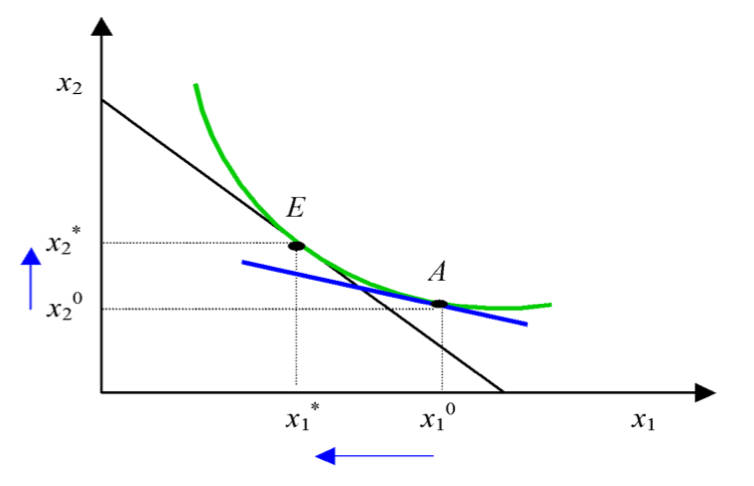
\includegraphics[width=12cm]{ayu1}
				\scriptsize{\newline \emph{Fuente:}Construcci�n del autor}
			\end{figure}
			\smallskip.
	
\end{enumerate}

\begin{enumerate}
	\item Considere un consumidor con preferencias estrictamente convexas. El valor absoluto de la pendiente de una curva de indiferencia en el punto $(x_{1} = 3, x_{2} = 4)$ es 2. 
	
	\begin{enumerate}[(a)]
		\item �Cuanto vale el valor absoluto de dicha pendiente cuando $x_{2}$ = 2?
	\end{enumerate}
\end{enumerate}

\bigskip
{\Large Soluci�n}
\bigskip

\begin{enumerate}[(a)]
	\item Cuando las preferencias son estrictamente convexas las curvas de indiferencia son continuamente decrecientes y verifican:
	$$\frac{\partial \arrowvert RMS_{x_{1},x_{2}}\arrowvert}{\partial x_{1}}<0$$
	
Por lo tanto, partiendo de la cesta $(3,4)$, si se reduce la cantidad de $x_{2}$, para mantenernos sobre la misma curva de indiferencia, ya que  �sta tiene pendiente negativa, pasaremos a una cesta que contendr� necesariamente una cantidad mayor de $x_{1}$, por lo cual se reducir� el valor absoluto de la pendiente de la curva de indiferencia en la nueva cesta, siendo menor que 2. Gr�ficamente, si el individuo parte de la cesta A, pasar� a una cesta situada a su derecha como por ejemplo la B:
 
	\begin{figure} [h!]
		\centering
		\caption{\textbf{Soluci�n pregunta 2.}}
		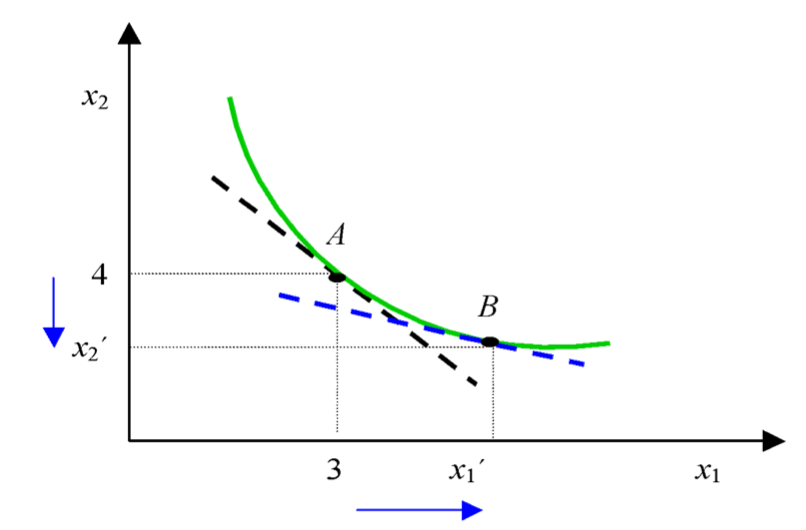
\includegraphics[width=12cm]{ayu2}
		\scriptsize{\newline \emph{Fuente:}Construcci�n del autor}
	\end{figure}
	\smallskip.
	
\end{enumerate}

\end{document}

